\begin{frame}{CW-Complejos}
Un CW-complejo es un tipo particular de espacio topológico muy útil en la teoría de homotopía.
Construimos los espacios llamados $n$-esqueletos:
\[ X^0 \subset X^1 \subset \ldots \subset X^n \subset \ldots \]
 Definimos entonces el CW-complejo como $\displaystyle X = \bigcup_{n \geq 0} X^n$.
\end{frame}

\begin{frame}{CW-Complejos}
Un ejemplo de CW-complejo es la esfera $S^n$. Tenemos dos construcciones posibles:
\begin{tabular}{ll}
\begin{minipage}{0.5\textwidth}
\centering
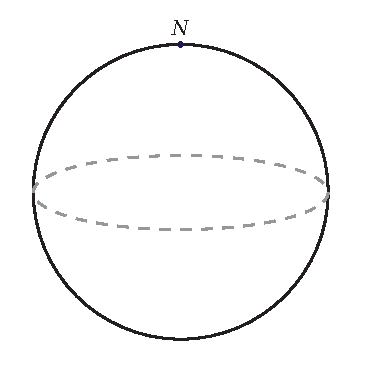
\includegraphics[width = 0.6\textwidth]{images/cwesfera1}
\par
En esta descomposición, tomamos una $0$-celda y una $n$-celda.
\end{minipage}
& \pause
\begin{minipage}{0.5\textwidth}
\centering
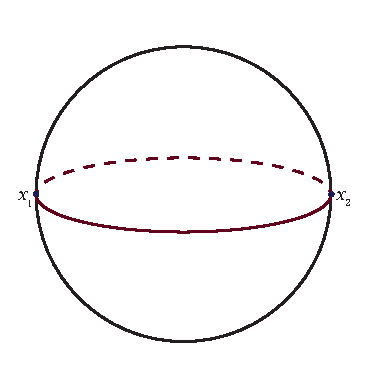
\includegraphics[width = 0.6\textwidth]{images/cwesfera2}
\par
Descomponemos la esfera en dos $0$-celdas, dos $1$-celdas, dos $2$-celdas...
\end{minipage}
\end{tabular}
\end{frame}

\begin{frame}{CW-Complejos}
Una superficie orientable compacta $M_g$ de género $g$ está compuesta por una $0$-celda, $2g$ $1$-celdas y una $2$-celda.
\begin{figure}
\centering
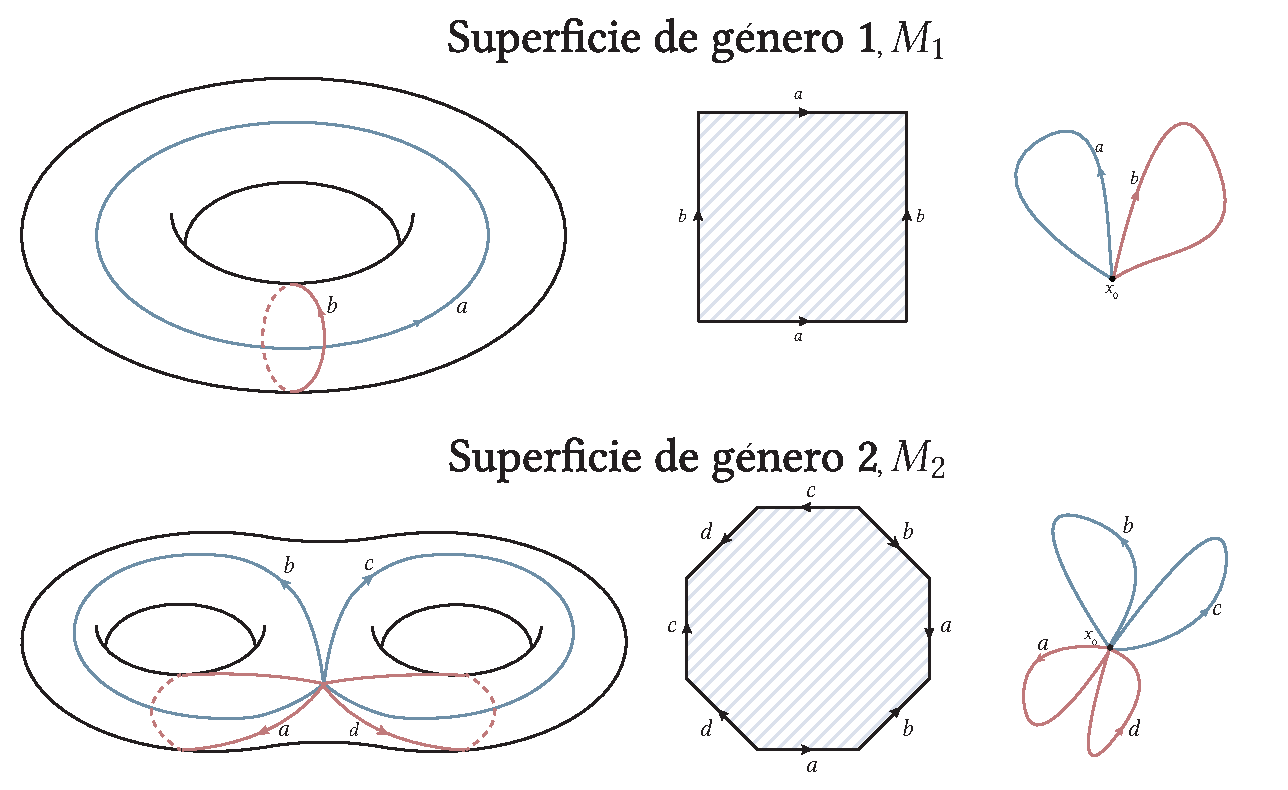
\includegraphics[width = 0.7\textwidth]{images/supgeng}
\end{figure}
\end{frame}

%\begin{frame}{CW-complejos}
% El espacio proyectivo real $\mathbb{R}P^n$ está compuesto por una $k$-celda de cada orden hasta grado $n$.
%\begin{figure}
%\centering
%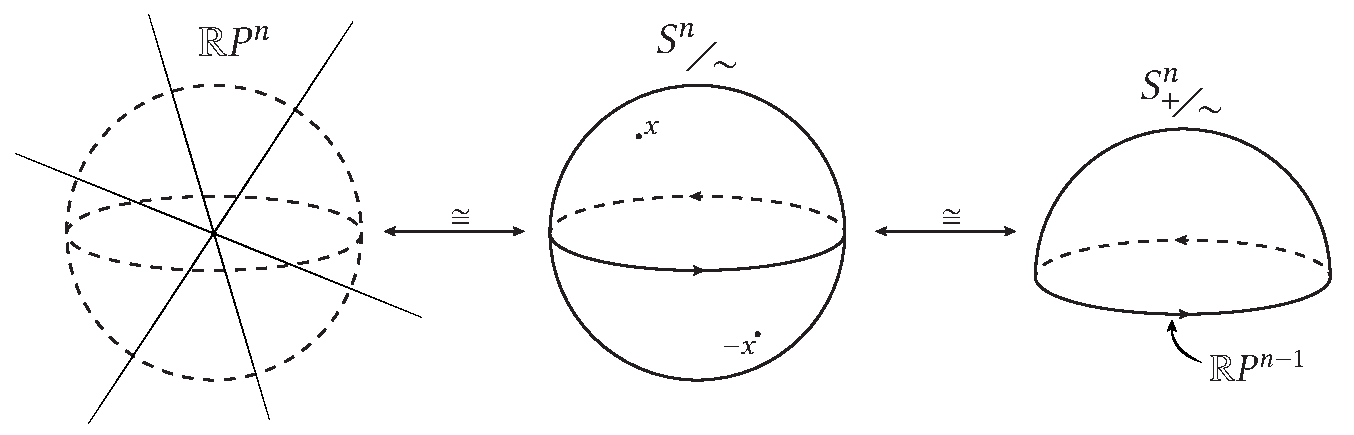
\includegraphics[width = 0.7\textwidth]{images/proyecreal}
%\end{figure}
%\end{frame}

\begin{frame}{Suspensión y espacio de lazos}
\begin{defin}
Dado un espacio topológico $X$, se define la suspensión de $X$ como
\begin{tabular}{ll}
\begin{minipage}{0.5\textwidth}
\[ \Sigma X =  \faktor{X \times I}
{ \footnotesize{\begin{matrix}
(x, 1) \sim (x', 1) \\
(x, 0) \sim (x', 0)
\end{matrix}}} \] 
\end{minipage}
&
\begin{minipage}{0.5\textwidth}
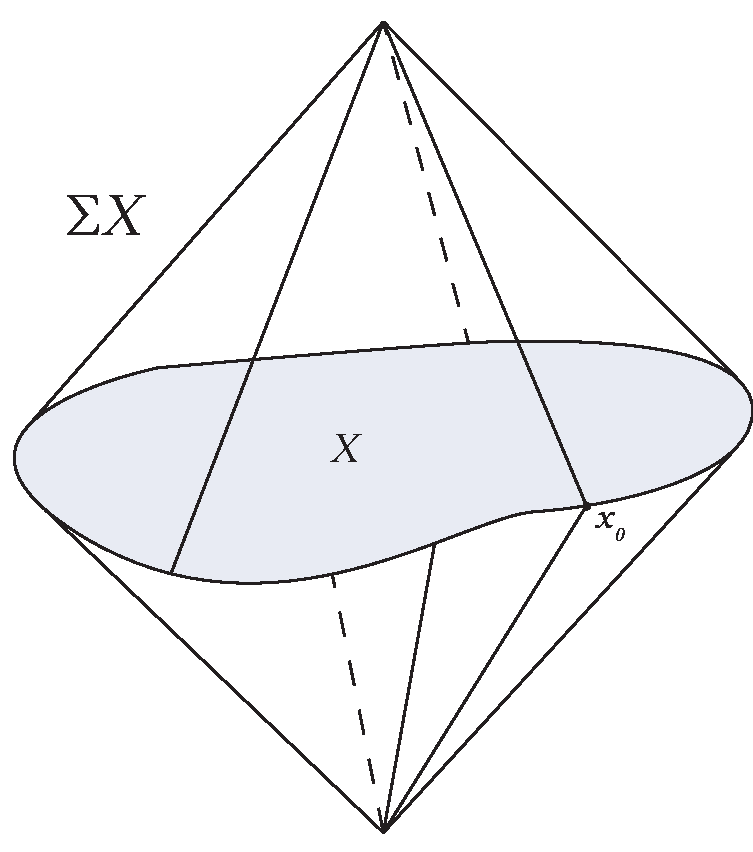
\includegraphics[width=0.4\textwidth]{images/suspension.pdf}
\end{minipage}
\end{tabular}
\end{defin}
\pause
\begin{defin}
Se define el espacio de lazos de $X$ como
\[
\Omega X = (X, x_0)^{(S^1, \ p_0)} = \{ f : I \longrightarrow X \ \vert \ f(0) = f(1) = x_0 \}
\]
\end{defin}
\end{frame}
\begin{frame}{Suspensión y espacio de lazos}
\begin{teor}
Sean $X$ e $Y$ dos espacios punteados cualesquiera. Entonces
$[X, \Omega Y]$ y $[\Sigma X, Y]$ son grupos. Además,
\[ [X, \Omega Y] \cong [\Sigma X, Y] \]
\end{teor}

\end{frame}